Se comenz� por emular un sistema de segundo orden  que permitiera obtener el comportamiento de la planta, para esto se tomo el sistema de un motor de segundo orden que cumple con las ecuaciones mostradas en \ref{ec:motorarmadura}.

Las cuales se pueden organizar de la siguiente forma:
 \begin{center}
 \begin{equation}
 	\left\{
	\begin{matrix}
		&\dot{W}_{M}=I_{M}\left ( \frac{K_{M}}{J_{M}} \right )-W_{M}\left (\frac{F_{M} }{J_{M}}\right )\\
		& \dot{I_{M}} = V_{M}\left ( \frac{1}{L_{M}} \right )-I_{M}\left ( \frac{R_{M}}{L_{M}} \right )-W_{M}\left (  \right \frac{1}{L_{M}} )
    \end{matrix}
\right.
		\label{ec:motorarmadura2}%
		%\textup{Ecuaciones de un motor DC controlado por armadura}	
	\end{equation}
\end{center}
 Se busco un sistema  estudio el sistema "The DC Motor Control Trainer" (DCMCT), conocido como Quanser y como nos referiremos a el a partir de ahora y el cual cumple con los siguientes par�metros presentados en el manual de uso del dispositivo
 
  \begin{figure}[H]
 	\centering
 	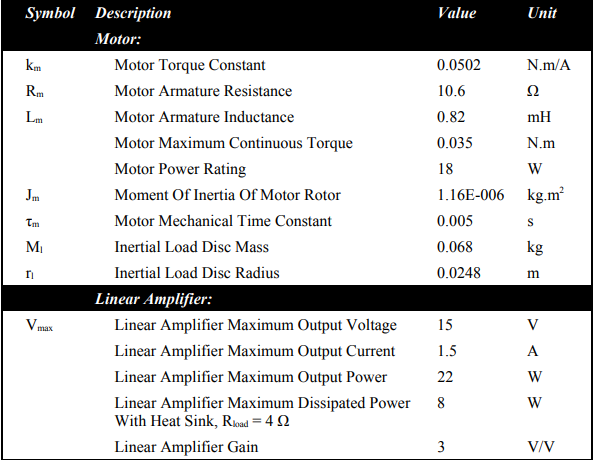
\includegraphics[width=1\linewidth]{img/quanser}
 	\caption{Par�metros Quanser}
 	\label{fig:Quanser}
 	\cite{q}
 \end{figure}  
 
 
 Se tomo los par�metro $ J_{m}$ del Quanser para calcular el $ J_{equi}$, despreciando la fricci�n y usando los Siguientes par�metros $M_{l}=0.068kg$ y $r_{l}=0.0248m$
 
 \begin{center}
 	\begin{equation}
 		J_{equi}=J_{m}+J_{l}\left ( \frac{R_{eje}}{R_{l}} \right )
 	\end{equation}
\end{center}

Donde $ J_{l}=\frac{M_{l}r_{l}^{2}}{2}$ y donde las relaciones entre los radios es de 1.



\begin{center}
	\begin{equation}
		J_{equi}=J_{m}+\frac{M_{l}r_{l}^{2}}{2}
	\end{equation}
\end{center}

Obteniendo los par�metros de \ref{ec:valoresmotorarmadura} que se tomaran para emular la planta   
 \begin{center}
	 \begin{equation}
		\begin{matrix}
			K_{M}=0.0502\frac{Nm}{A}\\ 
			J_{equiv}= 21,4567*10^{-6} Kg.m^{2}\\ 
			R_{m}=10.6\Omega\\ 
			L_{m}=0.82m H	
		\end{matrix}
		 \label{ec:valoresmotorarmadura}%
	\end{equation}
\end{center}

El sistema de segundo orden que se intenta emular es el Quanser la cual cumple con las caracter�sticas anteriores, para as� poder realizar las pruebas necesarias para evaluar el comportamiento de la planta con un controlador real. Al realizar el espacio de estado de la planta se obtiene

\begin{center}
	\begin{equation}
		\left\{\begin{matrix}
			\begin{bmatrix}
				& \dot{W_{M}}\\ 
				& \dot{I_{M}}
			\end{bmatrix}
			=
			\begin{bmatrix}
				& \frac{-F_{M}}{J_{M}} & \frac{K_{M}}{J_{M}} & \\ 
				&  \frac{-K_{M}}{L_{M}}& \frac{-R_{M}}{L_{M}} & \\ 
			\end{bmatrix}
			\begin{bmatrix}
				& W_{M} \\ 
				& I_{M}
			\end{bmatrix}
			+
			\begin{bmatrix}
				& 0 \\ 
				& \frac{1}{L_{M}}
			\end{bmatrix}
			V_{M}\\ 
			Y=\begin{bmatrix}
				1 & 0
			\end{bmatrix}
			\begin{bmatrix}
				W_{M}\\ 
				I_{M}
			\end{bmatrix}
		\end{matrix}\right.	
    \end{equation}
\end{center}

\begin{center}
	\begin{equation}
		\left\{\begin{matrix}
			\begin{bmatrix}
				& \dot{W_{M}}\\ 
				& \dot{I_{M}}
			\end{bmatrix}
			=
			\begin{bmatrix}
				& 0 & 2340 & \\ 
				&  -61,22& -1,293.10^{4} & \\ 
			\end{bmatrix}
			\begin{bmatrix}
				& W_{M} \\ 
				& I_{M}
			\end{bmatrix}
			+
			\begin{bmatrix}
				& 0 \\ 
				& 1220
			\end{bmatrix}
			V_{M}\\ 
			Y=\begin{bmatrix}
				1 & 0
			\end{bmatrix}
			\begin{bmatrix}
				W_{M}\\ 
				I_{M}
			\end{bmatrix}
		\end{matrix}\right.	
	\end{equation}
\end{center}

Para una planta de segundo orden gen�rica se tiene la ecuaci�n \ref{ec:plantasegundo}
\begin{center}
	\begin{equation}
		\frac{Y(s)}{U(s)}= \frac{b_{2}s^{2}+b_{1}S+b_{0}}{a_{2}S^{2}+a_{1}S+a_{0}} 
		\label{ec:plantasegundo}%
	\end{equation}
\end{center}

Como se pudo observar los motores de segundo orden que se van a estudiar tienen los valores de $b_{1}=0$ y $b_{2}=0 $ entonces la ecuaci�n quedar�a 

\begin{center}
	\begin{equation}
		\frac{Y(s)}{U(s)}= \frac{b_{0}}{a_{2}S^{2}+a_{1}S+a_{0}} 
		\label{ec:plantasegundo}%
	\end{equation}
\end{center}

Resolviendo las ecuaciones diferenciales se tiene que 

\begin{center}
	\begin{equation}
		\begin{matrix}
		a_{2}\ddot{y}+a_{1}\dot{y}+a_{0}y=b_{0}U \\
	 	x_{1}=y\\
		\dot{x_{1}}=\dot{y}=\dot{x_{2}}\\
		\ddot{x_{1}}=\ddot{y}=x_{3}\\
		\label{ec:solecdiferencial2}%
		\end{matrix}
	\end{equation}
\end{center}

Obteniendo el siguiente espacio de estado

\begin{center}
	\begin{equation}
		\begin{bmatrix}
			\dot{x_{1}}\\
			\dot{x_{2}}
		\end{bmatrix}
		=
		\begin{bmatrix}
			0 & 1\\ 
			-\frac{a_{0}}{a_{2}}& -\frac{a_{1}}{a_{2}}
		\end{bmatrix}x+
		\begin{bmatrix}
			0\\ 
			\frac{b_{0}}{a_{2}}
		\end{bmatrix}
		\label{ec:espaciodestado2}%
	\end{equation}
\end{center}

\section{Dise�ar la interfaz de emulaci�n de la planta de segundo orden}

La plataforma tecnol�gica que se selecciono fue Python la cual cumple con todas las requisitos requeridos en el capitulo \ref{CAP:tecni}, y con las librer�as explicadas en la secci�n de Python.

Se utilizo la interfaz gr�fica tkinter la cual se configuro para que se pudieran cambiar los t�rminos que componen a la ecuaci�n de la planta  planteada de segundo orden, aunque se preestablecio los datos para el funcionamiento del Quanser, los elementos se pueden cambiar para que se pueda emular cualquier planta de segundo orden que cumpla con la ecuaci�n dada en \ref{ec:plantasegundo}


Se habilito otra entrada para poder insertar el puerto por el cual se va a realizar la comunicaci�n serial con el controlador real y un bot�n para conectarlo donde nos saldr� un mensaje de si la comunicaci�n fue correcta o ocurri� un error en el proceso.

Se cuenta con un bot�n para iniciar la comunicaci�n con el controlador y dos botones uno para graficar la respuesta controlada y otro para ver la respuesta original.
 
Por �ltimo se mostrar� los datos de sobrepico porcentual, tiempo de establecimiento y tiempo de alza.

 